\documentclass[11pt, a4paper, UKenglish]{article}
\usepackage[T1]{fontenc}
\usepackage{lmodern}
\usepackage[utf8]{inputenc}
\usepackage{tabularx}
\usepackage{mathtools}
\usepackage{color}
%%%%%%%%%%%%%%%%%%%%%%%%%%%%%%%%%%%%%%%%%%%%%%%%
% load packages
\usepackage{amsmath}   % for more basic mathematical symbols
\usepackage{amssymb}   % for more mathematical symbols
\usepackage{amsthm}
\usepackage{tikz-cd}
\usepackage{tikz}
\usetikzlibrary{3d,calc,intersections}
\usetikzlibrary{arrows.meta}
\usetikzlibrary{decorations.markings}
\usetikzlibrary{patterns}
\usetikzlibrary{quotes,angles,positioning}
\usepackage{dsfont}
\usepackage{ stmaryrd }
\usepackage{caption}
\usepackage[final]{listings}


\newtheorem{theorem}{Theorem}
\newtheorem{lemma}{Lemma}
\newtheorem*{remark}{Anmerkung}
\newtheorem{definition}{Definition}
\newcommand{\bK}{\mathbb{K}}
\newcommand{\bN}{\mathbb{N}}
\newcommand{\bZ}{\mathbb{Z}}
\newcommand{\bR}{\mathbb{R}}
\newcommand{\bC}{\mathbb{C}}
\newcommand{\bS}{\mathbb{S}}
\newcommand{\bA}{\mathbb{A}}
\newcommand{\bB}{\mathbb{B}}
\newcommand{\bD}{\mathbb{D}}
\newcommand{\bE}{\mathbb{E}}
\newcommand{\bT}{\mathbb{T}}
\newcommand{\bQ}{\mathbb{Q}}

\newcommand{\im}{\textrm{im}}
\newcommand{\coker}{\textrm{coker}}
%%%%%%%%%%%%%%%%%%%%%%%%%%%%%%%%%%%%%%%%%%%%%%%%%%%%%%%

\renewcommand{\figurename}{Fig.}

\newcolumntype{L}[1]{>{\raggedright\arraybackslash}p{#1}}
%Linksbündig mit vorgegebener Breite
\newcolumntype{C}[1]{>{\centering\arraybackslash}p{#1}}
%Zentriert mit vorgegebener Breite
\newcolumntype{R}[1]{>{\raggedleft\arraybackslash}p{#1}}
%Rechtsbündig mit vorgegebener Breite

\usepackage{BA_Titelseite}

%Namen des Verfassers der Arbeit
\author{Jacobus Leander Conradi\\Vincent Reinthal}
%Datum der Abgabe der Arbeit
\date{\today}

%Name des Betreuers
% z.B.: Prof. Dr. Peter Koepke
\betreuer{supervisor: Prof.\ Dr. Rolf Klein}
%Name des Instituts an dem der Betreuer der Arbeit tätig ist.
\zweitgutachter{secondary supervisor: Dr. Elmar Langetepe}
%Titel der Bachelorarbeit
\title{Wasserstein distance for persistence diagrams}
%Do not change!
\ausarbeitungstyp{Lab Report}

\usepackage{afterpage}

\newcommand\blankpage{%
\null
\thispagestyle{empty}%
\addtocounter{page}{-1}%
\newpage}

\definecolor{dkgreen}{rgb}{0,0.6,0}
\definecolor{gray}{rgb}{0.5,0.5,0.5}
\definecolor{mauve}{rgb}{0.58,0,0.82}

\lstset{language=Java,
aboveskip=2mm,
belowskip=2mm,
showstringspaces=false,
columns=flexible,
basicstyle={\small\ttfamily},
numbers=none,
numberstyle=\tiny\color{gray},
keywordstyle=\color{blue},
commentstyle=\color{dkgreen},
stringstyle=\color{mauve},
breaklines=true,
breakatwhitespace=true,
tabsize=3
}


\begin{document}
    \maketitle

    \thispagestyle{plain}
    \pagenumbering{Roman}
    \addtocounter{page}{-1}
    \tableofcontents
    \addcontentsline{toc}{section}{Table of contents}
    \vfil\null
    \clearpage
    \thispagestyle{empty}\mbox{}
    \clearpage
    \pagenumbering{arabic}

    \section{The problem}\label{ch:the-problem}
    In this work we want to take a look at the comparison of different types of image data.
    For this we consider the concept of persistent homology.
    Persistent homology can best be described as the ''recognition of structure while squinting''.
    In essence, we want to reduce a complex-looking data set to basic geometric forms.
    In particular, this approach is very intuitive and close to the subconscious recognition of structures that are characteristic of a human.\\
    For a given data set we first want to calculate a so called persistence diagram and then find a suitable distance measure for such diagrams.


    \subsection{Persistent Homology}\label{sec:persistent-homology}

    In order to calculate homologies, we first need a manifold, or in the case of a computer a necessarily discrete representation, a cell complex.
    We begin by defining the cell complex, we will be working with, namely the Čech-complex for a given point set.

    \begin{definition}[Čech-Complex]
        Let $X\subset \bR^d$ be a finite set, and $\varepsilon>0$ arbitrary but fixed.
        We construct the Čech-complex $\check C_\varepsilon(X)$ as follows.
        The $0$-skeleton is simply $X$ itself.
        And any subset $\sigma\subset X$ is in the $(|\sigma|-1)$-skeleton iff the intersection $\bigcap_{x\in\sigma}B_\varepsilon(x)$ of balls with radius $\varepsilon$ around every point of $\sigma$ is non-empty.
    \end{definition}

    Note, that for any finite $X$ there is  $\mathcal{E}>0$, such that for any $\varepsilon\geq\mathcal{E}$ we have  $\check C_\varepsilon(X) = \check C_\mathcal{E}(X)$.
    Call this stabilizing cell-complex $C(X):=\check C_\mathcal{E}(X)$.
    Define a filtration $f$ on $C(X)$ via $f:C(X)\rightarrow\bR$, $\sigma\mapsto\min\{\varepsilon|\sigma\in \check C_\varepsilon(X)\}$.
    Since $X$ is finite, and hence $C(X)$, $\im(f)$ must also be finite.
    Let $\im(f)=\{\varepsilon_i|0\leq i\leq N\}$.
    We now get a sequence of cell-complexes \[\check C_{\varepsilon_1}(X)\hookrightarrow \check C_{\varepsilon_2}(X)\hookrightarrow \ldots \hookrightarrow \check C_{\varepsilon_{N-1}}(X)\hookrightarrow \check C_{\varepsilon_N}(X).\]
    With this sequence we will now define persistent Homology.

    \begin{definition}[persistent Homology]
        Let \[X_1\xhookrightarrow{\iota_1} X_2\xhookrightarrow{\iota_2} \ldots\xhookrightarrow{\iota_{n-2}} X_{n-1}\xhookrightarrow{\iota_{n-1}} X_n\] be a sequence of cell-complex embeddings.
        For every $k\geq 0$ this implies a sequence of homology groups
        \[H_k(X_1)\xrightarrow{\iota_{1}^*} H_k(X_2)\xrightarrow{\iota_{2}^*}\ldots \xrightarrow{\iota_{n-2}^*} H_k(X_{n-1})\xrightarrow{\iota_{n-1}^*} H_k(X_n).\]
        For every $0\leq i<j\leq n$ we begin with $\mathcal{L}_i^j(X)_k$ the set of generators $\sigma\in\coker(\iota_{i-1}^*)$, such that $\iota_{j-2}^*\circ\ldots\circ\iota_{i}^*(\sigma)\neq0$ but $\iota_{j-1}^*\circ\ldots\circ\iota_{i}^*(\sigma)=0$.
        Now to get the persistent homology from this, we need to apply the so called ''elder rule''.
        It may happen, that $\sigma_1\in\mathcal{L}_i^l(X)_k$ and $\sigma_2\in\mathcal{L}_j^l(X)_k$ exist (w.l.o.g. $i\leq j$), such that $\sigma_1$ equals $\sigma_2$ at some point $t$.
        In this case, we kill the ''younger'' one of the two, i.e.\ moving $\sigma_2$ to $\mathcal{L}_j^t(X)_k$, or removing completely, if $j=t$.
        We will call this reduced family $\{\mathcal{L}_i^j(X)_k|0\leq i<j\leq n,k\geq0\}$ the persistent homology of $\{X_i\}$.
    \end{definition}

    \begin{figure}
        \centering
        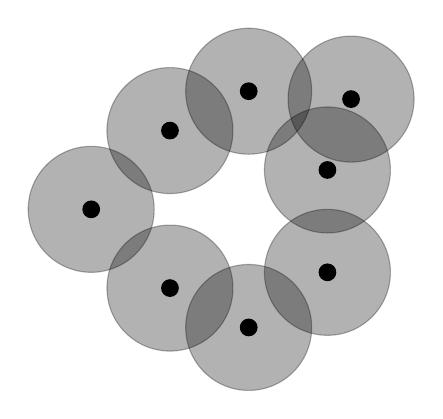
\begin{tikzpicture}
            \filldraw (0,0) coordinate(a) circle (3pt);
            \filldraw (-1,1) coordinate(b) circle (3pt);
            \filldraw (0.3,0.9) coordinate(c) circle (3pt);
            \filldraw (0,-1.3) coordinate(d) circle (3pt);
            \filldraw (-1,-2) coordinate(e) circle (3pt);
            \filldraw (-2,-1.5) coordinate(f) circle (3pt);
            \filldraw (-3,-0.5) coordinate(g) circle (3pt);
            \filldraw (-2,0.5) coordinate(h) circle (3pt);

            \filldraw[opacity=0.3] (a) circle (0.8);
            \filldraw[opacity=0.3] (b) circle (0.8);
            \filldraw[opacity=0.3] (c) circle (0.8);
            \filldraw[opacity=0.3] (d) circle (0.8);
            \filldraw[opacity=0.3] (e) circle (0.8);
            \filldraw[opacity=0.3] (f) circle (0.8);
            \filldraw[opacity=0.3] (g) circle (0.8);
            \filldraw[opacity=0.3] (h) circle (0.8);
        \end{tikzpicture}
        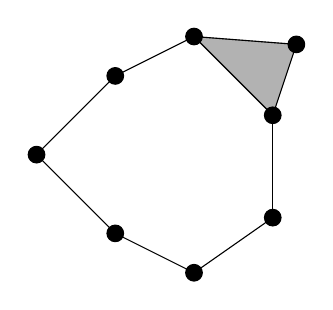
\begin{tikzpicture}
            \filldraw (0,0) coordinate(a) circle (3pt);
            \filldraw (-1,1) coordinate(b) circle (3pt);
            \filldraw (0.3,0.9) coordinate(c) circle (3pt);
            \filldraw (0,-1.3) coordinate(d) circle (3pt);
            \filldraw (-1,-2) coordinate(e) circle (3pt);
            \filldraw (-2,-1.5) coordinate(f) circle (3pt);
            \filldraw (-3,-0.5) coordinate(g) circle (3pt);
            \filldraw (-2,0.5) coordinate(h) circle (3pt);

            \draw (a) -- (b);
            \draw (a) -- (c);
            \draw (c) -- (b);

            \filldraw [opacity=0.3] (a) -- (b) -- (c);

            \draw (a) -- (d);
            \draw (d) -- (e);
            \draw (e) -- (f);
            \draw (f) -- (g);
            \draw (g) -- (h);
            \draw (h) -- (b);
        \end{tikzpicture}
        \caption{\textit{A Čech-Complex for a given $\varepsilon$ and generating point set.}}
    \end{figure}

    In essence persistent homology stores the lives and deaths of various generators, while increasing the maximum filtration value of elements in the cell complex.\\
    Since in this report we limit ourselves to $2$-dimensional point sets $X$, it is sufficient to limit the cell complex $C(X)$ to its $2$-complex, since all higher homologies vanish.

    One can geometrically define the calculation of these homologies for $2$-dimensional data as follows.
    Let balls grow evenly around each point of $X$.
    Unite these and calculate the homology of the resulting manifold.
    This creates ''holes'' at different times, i.e.\ generators of the first homology, which disappear again at large $\varepsilon$.\\
    We want to calculate this persistent homology for the Čech-Complex of given sets of points efficiently, and will take a look at different approaches to calculate these.
    \subsubsection{Persistence Diagrams}\label{subsec:persistence-diagrams}

    In order to work with persistent homology more intuitively we want to visualize these.
    A particular type of visualization we want to work with are called persistence diagrams.
    Here we want to mark the point $(t_1,t_2)$ in $\bR^2$ for every generator who is born at time $t_1$ and dies at time $t_2$.
    In more general terms, for every $\sigma\in\mathcal{L}_i^j(X)_k$ mark $(\varepsilon_i,\varepsilon_j)$ in $\bR^2$.
    \begin{figure}
        \centering
        \fbox{
        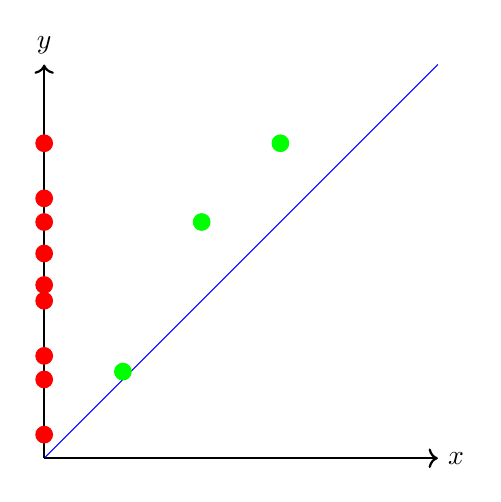
\begin{tikzpicture}
            % Achsen zeichnen
            \draw[->,thick] (0,0) -- (5,0) node[right] {$x$};
            \draw[color=blue] (0,0) -- (5,5);
            \draw[->,thick] (0,0) -- (0,5) node[above] {$y$};
            %Punkte einzeichnen:

            \filldraw[color=red] (0,0.3) coordinate(a) circle (3pt);
            \filldraw[color=red] (0,1) coordinate(a) circle (3pt);
            \filldraw[color=red] (0,1.3) coordinate(a) circle (3pt);
            \filldraw[color=red] (0,3) coordinate(a) circle (3pt);
            \filldraw[color=red] (0,4) coordinate(a) circle (3pt);
            \filldraw[color=red] (0,3.3) coordinate(a) circle (3pt);
            \filldraw[color=red] (0,2) coordinate(a) circle (3pt);
            \filldraw[color=red] (0,2.2) coordinate(a) circle (3pt);
            \filldraw[color=red] (0,2.6) coordinate(a) circle (3pt);


            \filldraw[color=green] (2,3) coordinate(a) circle (3pt);
            \filldraw[color=green] (1,1.1) coordinate(a) circle (3pt);
            \filldraw[color=green] (3,4) coordinate(a) circle (3pt);

        \end{tikzpicture}
        }
        \caption{\textit{A persistence-diagram.
        Red dots represent the $0$th, green dots the $1$st homology}}
        \label{fig2}
    \end{figure}

	Note that the points marked in this way are always above the diagonal $\Delta=\{(x,x)\in\bR^2|x\in\bR\}$, where points directly on the diagonal represent generators that die quickly after birth, and points far from the diagonal represent generators that live very long.
    Fig.~\ref{fig2} is an example for a persistence diagram which shows ''holes'' at three different times, i.e.\ generators of the first homology.
    Furthermore, one can see that the generators of the zeroth homology - i.e.\ one per connected component at every point in time - are all born at time 0.\\
    \subsection{Wasserstein Distance}\label{sec:wasserstein-distance}

    Now let two such persistence diagrams be given.
    To define a distance measure, we consider the Wasserstein distance often used in probability theory.
    This is the ''minimum effort to move one probability distribution to another''.
    In our concrete application we define this as follows.

    \begin{definition}[Wassersteindistanz]
        Let two finite pointsets $X$ and $Y$ be given, with $|X|=|Y|$.
        Then the Wasserstein distance is given by\[W_p(X,Y) = \min_{\varphi:X\rightarrow Y}\left(\sum_{x\in X}||x-\varphi(x)||^p\right)^{\frac{1}{p}},\]
        where the minimum is taken over all bijections $\varphi:X\rightarrow Y$, with $||\cdot||$ being the $\ell_2$-norm in $\bR^2$.
    \end{definition}

    A special case $W_\infty(\cdot,\cdot)$ we will call the Bottleneck distance.\\
    Notice the restraint $|X| = |Y|$.
    We want to adapt this such that differently sized sets can be compared with each other as well.
    For this we want to compare different approaches qualitatively.

    \subsection{Feature Proposals}\label{sec:feature-proposals}

    As a final step, we will examine methods to find a representative set of points $X$ for a given image to use as input for calculating persistent homology.
    Again, we want to compare different methods and compare them in the context of persistent homology.
    \section{Persistent Homology}\label{ch:persistent-homology}

    In this chapter we want to focus on the implementation for the computation of the Čech complex, as well as the calculation of persistent homology and persistence diagrams.

    \subsection{Computation of the Čech-Complex}\label{sec:čech-complex}

    To calculate the Čech complex we first look at the Voronoi diagram for a given point set $X$ in $2$-dimensional space.
    Here $\bR^2$ is divided into regions, so that in each region there is exactly one point $x$ of $X$, and for every other point $y$ of this region $x$ is the nearest point of $X$ to $y$.\\
    From the Voronoi diagram we can extract the Čech complex.
    We add an edge between $x$ and $y$ from $X$ to the cell complex when the Voronoi regions of $x$ and $y$ meet.
    The distance of $x$ and $y$ also gives us the filtration value $f(\{x,y\}) = \frac{||x-y||}{2}$ of the edge.
    If you add all these edges, you get the planar dual-graph, the DeLauney triangulation of the points from $X$.\\
    It gets more complicated with faces, i.e. $2$-cells.
    Here we have to make an important case distinction.
    If more than $2$ Voronoi regions touch in a point, this corresponds to a circuit in the DeLauney trinagulation and a $2$-cell in the Čech complex.
    But what exactly is the filtration value?
    This is where the following case distinction comes into play.
    Looking at the convex hull of the points $x_1,\ldots,x_k\in X$, whose Voronoi regions touch each other, it can happen that the point $v$ where the Voronoi regions touch each other is inside or outside the convex hull.
    If the point $v$ is inside the convex hull, the filtration value must be chosen as the distance of $v$ to all $x_i$, which is the same for all $x_i$.
    Because as soon as this value is exceeded, the hole in the geometric presentation vanishes, hence the face must be inserted into the complex.\\
    \lstset{language=Java}
\begin{figure}
    \begin{lstlisting}[frame=single]
        public class Voronoi {
            // Stores voronoi vertices, where more than 2 regions touch
            private PointD[] vertices = null;
            private VEdge[] edges = null;
            ...
            private void compute(int width, int height) {
                 VoronoiResults results = org.kynosarges.tektosyne.geometry.Voronoi.findAll(
                 sites, new RectD(0, 0, width, height));
                 vertices = results.voronoiVertices;
                 // Transform output of library to our own data types
            ...
            }
            ...
        }
        public class ActionGenerator {
            public List<Action> generate() {
                // Generate the list of elements added to the cell complex sorted by their filtration values
                ...
                voronoi.forEachVertex(this::computeVertex);
                voronoi.forEachEdge(this::computeEdge);
                actions.sort(Action::compareTo);
                return actions;
            }
            private void computeVertex(@NotNull PointD vertex, int index) {
                // Create list of actions given the Voronoi Diagram
                ...
                VEdge[] edges = voronoi.getEdges(edgeIndices);
                PointD[] sites = getSites(edges);
                if (Util.isInside(vertex, sites)) {
                    actions.add(new FaceAction(...));
                    return;
                }
                ...
                actions.add(new EdgeFaceAction(...));
            }
        }
    \end{lstlisting}
    \caption{\textit{Codesnippet of the generation of $C(X)$}}
    \label{fig3}
\end{figure}
    In the other case, there is no point in time where the circuit given by the points $x_1,\ldots,x_k$ in the geometric representation is ''around a hole'' - i.e.\ never is a generator -, so the face must be inserted as soon as the last edge closes the circle in $x_1,\ldots,x_k$.
    In other words, the filtration value is $\max f(\{x_i,x_{i+1}\})$.
    We want to call these $2$-cells \textit{degenerated}.
    For the implementation in Java we decided to use a library which calculates the Voronoi diagram.
    We calculate the planar dualgraph based on the library, as shown in Fig.~\ref{fig3} Furthermore, we see that in the case of degenerated $2$-faces we use a \texttt{EdgeFaceAction} to insert the longest edge of the circle and the $2$-cell in the same time step.

    \subsection{Calculation of persistent Homology}\label{sec:calculation-of-persistent-homology}

    Since the $1$-skeleton is the same as a graph, we save the complex as a graph, and remember which relations are generated by $2$-cells.
    And because the second homology is always zero, due to our choice of $2$-dimensional data, this suffices.

    To respect the ''elder rule'', we need to make a choice for $0$-cells which vertices are older than other vertices.
    Since the choice has no influence on the zero homology persistence diagram, we number the vertices randomly.
    We use this numbering when calculating the first homology as an orientation of the edges.

    The main task in our implementation is the calculation of the first homology.
    For the zeroth homology we only have to remember whenever we add an edge whether the two vertices are in the same or different connected components.
    To maintain the elder rule for generators, we remember for each node which is the oldest one in each connected component.
    If the added edge is between two different connected components, we update for one of the connected components which the new oldest vertex is, and remember that a generator of the zeroth homology has died.

    Since generators of the first homology live in the kernel of the boundary operator $H_1(C(X))\rightarrow H_0(C(X))$, and these are just described by all circuits, we must find all possible circles in the graph, and then find out which circuits die via linear combinations of these.
    To find circuits, we check whenever we add an edge $e=(v,w)$ whether $v$ and $w$ are in the same connected component.
    If this is the case, we find a $v,w$-path $P$ in $G\setminus \{e\}$.
    Then we remember $P\cup \{e\}$ as a new generator.
    At the time this generator is added, $e$ is completely new and is not yet contained in any edge of a $2$ cell or other circle, so this circle is definitely a living generator for a little time at least.

    If a $2$-cell is added, a relation is noted, namely the unique circle that describes the border of the $2$ cell.
    Every time a $2$-cell is added, we have to check if a circle dies.
    For this we check the kernel of the matrix:

    %$$\begin{matrix}
    %a & b\\
    %c & d
    %\end{matrix}$$

    \[\begin{Bmatrix}
          c_{11} & c_{21} & \ldots &c_{n1} & r_{11} & \ldots  & r_{k1}\\
          c_{12} & c_{22} & \ldots &c_{n2} & r_{12} & \ldots  & r_{k2}\\
          \vdots & \vdots & \ddots & \vdots & \vdots & \ddots & \vdots \\
          c_{1m} & c_{2m} & \ldots &c_{nm} & r_{1m} & \ldots  & r_{km}
    \end{Bmatrix}\]

    Where $c_{ij} = \sum_{e_j\in P_i} 1 - \sum_{e_j*\in P_i}1$ and $r_{ij} = \sum_{e_j\in R_i} 1 - \sum_{e_j^*\in R_i}1$, where $P_i$ is the generator circuits and $R_i$ is the relation circuits, and $e_j$ is an edge and $e_j^*$ is the inverted edge.

    \begin{figure}
        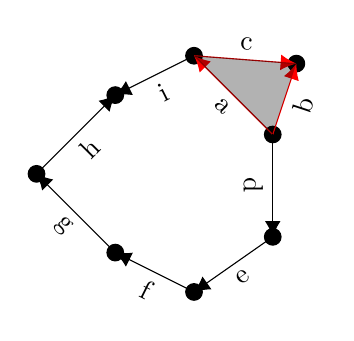
\begin{tikzpicture}
            \filldraw (0,0) coordinate(a) circle (3pt);
            \filldraw (-1,1) coordinate(b) circle (3pt);
            \filldraw (0.3,0.9) coordinate(c) circle (3pt);
            \filldraw (0,-1.3) coordinate(d) circle (3pt);
            \filldraw (-1,-2) coordinate(e) circle (3pt);
            \filldraw (-2,-1.5) coordinate(f) circle (3pt);
            \filldraw (-3,-0.5) coordinate(g) circle (3pt);
            \filldraw (-2,0.5) coordinate(h) circle (3pt);

            \draw [-{Latex[length=2mm,width=2mm]},color=red] (a) -- (b) node[midway,below,sloped,color=black]{a};
            \draw [-{Latex[length=2mm,width=2mm]},color=red](a) -- (c)node[midway,below,sloped,color=black]{b};
            \draw [-{Latex[length=2mm,width=2mm]},color=red](b) -- (c)node[midway,above,sloped,color=black]{c};

            \filldraw [opacity=0.3] (a) -- (b) -- (c);

            \draw[-{Latex[length=2mm,width=2mm]}] (a) -- (d)node[midway,below,sloped,color=black]{d};
            \draw[-{Latex[length=2mm,width=2mm]}] (d) -- (e)node[midway,below,sloped,color=black]{e};
            \draw[-{Latex[length=2mm,width=2mm]}] (e) -- (f)node[midway,below,sloped,color=black]{f};
            \draw[-{Latex[length=2mm,width=2mm]}] (f) -- (g)node[midway,below,sloped,color=black]{g};
            \draw[-{Latex[length=2mm,width=2mm]}] (g) -- (h)node[midway,below,sloped,color=black]{h};
            \draw[-{Latex[length=2mm,width=2mm]}] (b) -- (h)node[midway,below,sloped,color=black]{i};
        \end{tikzpicture}
        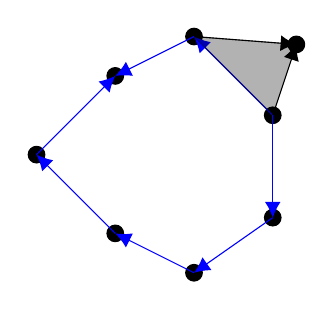
\begin{tikzpicture}
            \filldraw (0,0) coordinate(a) circle (3pt);
            \filldraw (-1,1) coordinate(b) circle (3pt);
            \filldraw (0.3,0.9) coordinate(c) circle (3pt);
            \filldraw (0,-1.3) coordinate(d) circle (3pt);
            \filldraw (-1,-2) coordinate(e) circle (3pt);
            \filldraw (-2,-1.5) coordinate(f) circle (3pt);
            \filldraw (-3,-0.5) coordinate(g) circle (3pt);
            \filldraw (-2,0.5) coordinate(h) circle (3pt);

            \draw [-{Latex[length=2mm,width=2mm]},color=blue] (a) -- (b);
            \draw [-{Latex[length=2mm,width=2mm]}](a) -- (c);
            \draw [-{Latex[length=2mm,width=2mm]}](b) -- (c);

            \filldraw [opacity=0.3] (a) -- (b) -- (c);

            \draw[-{Latex[length=2mm,width=2mm]},color=blue] (a) -- (d);
            \draw[-{Latex[length=2mm,width=2mm]},color=blue] (d) -- (e);
            \draw[-{Latex[length=2mm,width=2mm]},color=blue] (e) -- (f);
            \draw[-{Latex[length=2mm,width=2mm]},color=blue] (f) -- (g);
            \draw[-{Latex[length=2mm,width=2mm]},color=blue] (g) -- (h);
            \draw[-{Latex[length=2mm,width=2mm]},color=blue] (b) -- (h);
        \end{tikzpicture}
        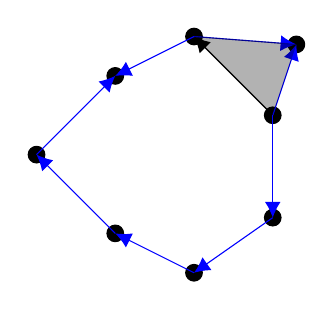
\begin{tikzpicture}
            \filldraw (0,0) coordinate(a) circle (3pt);
            \filldraw (-1,1) coordinate(b) circle (3pt);
            \filldraw (0.3,0.9) coordinate(c) circle (3pt);
            \filldraw (0,-1.3) coordinate(d) circle (3pt);
            \filldraw (-1,-2) coordinate(e) circle (3pt);
            \filldraw (-2,-1.5) coordinate(f) circle (3pt);
            \filldraw (-3,-0.5) coordinate(g) circle (3pt);
            \filldraw (-2,0.5) coordinate(h) circle (3pt);

            \draw [-{Latex[length=2mm,width=2mm]}] (a) -- (b);
            \draw [-{Latex[length=2mm,width=2mm]},color=blue](a) -- (c);
            \draw [-{Latex[length=2mm,width=2mm]},color=blue](b) -- (c);

            \filldraw [opacity=0.3] (a) -- (b) -- (c);

            \draw[-{Latex[length=2mm,width=2mm]},color=blue] (a) -- (d);
            \draw[-{Latex[length=2mm,width=2mm]},color=blue] (d) -- (e);
            \draw[-{Latex[length=2mm,width=2mm]},color=blue] (e) -- (f);
            \draw[-{Latex[length=2mm,width=2mm]},color=blue] (f) -- (g);
            \draw[-{Latex[length=2mm,width=2mm]},color=blue] (g) -- (h);
            \draw[-{Latex[length=2mm,width=2mm]},color=blue] (b) -- (h);
        \end{tikzpicture}
        \caption{An example for generators, that die, due to a relation. In red is the boundary of a $2$-cell, in blue are two generators that are identified with each other via the $2$-cell.}
        \label{fig4}
    \end{figure}

    An example in Fig.~\ref{fig4}.
    We are given two circles in blue, and a relation in red.
    If we number the edges as in the first picture and select all circle orientations counter clockwise we get the following matrix:
    \[A=\begin{Bmatrix}
            1 & 0 & -1\\
            0 & 1 & 1\\
            0 & -1 & -1\\
            -1 & -1 & 0\\
            -1 & -1 & 0\\
            -1 & -1 & 0\\
            -1 & -1 & 0\\
            -1 & -1 & 0\\
            1 & 1 & 0
    \end{Bmatrix}\]
    And thus get a non-empty kernel, $A(1,1,-1)^T=0$. So we know that the two generators are identified with each other and can remove the younger one out of the generator list.

    We now know when to add edges and faces and how to find all possible generators and how to find ''dead'' generators.
    Putting this together we are now able to calculate the first persistent homology.

    \subsubsection{Optimizations}\label{subsec:optimizations}

    Since this algorithm is not that efficient ($\sim5$ seconds for $100$ nodes, $\sim20$ seconds for $200$ nodes) we optimised it using contractions on the graph and get almost linear runtime ($\sim10$ seconds for $1000$ nodes).
    The main idea here is to not maintain a list of relations rather than handling the effect of relations as operation on the underlying graph.
    That removes the necessity of computing kernels of a growing matrix in each face step, but is not trivial to implement due to special cases in face contractions.\\
    Let us recap first.
    We have generated a list of actions, that are of exactly 3 different types:
    \begin{itemize}
        \item Edge actions: These add exactly one edge between two nodes.
        \item Face actions: These add a relation, that is going along a face, representing the face being contracted.
        \item Edge-face actions: These exist for degenerate faces and first add an edge of a face and then contract it.
    \end{itemize}
    Since we are going to add and remove edges, we first have to make sure, that we are sorting the actions in a way, that edges are only removed, after being added.
    Logically this should be an implication by the action generation using the Voronoi diagram, but in reality there are sometimes numerical problems, that destroy this order.
    To do this, we compute a dependency tree, where a face or edge-face action is depending on each edge or edge-face action, that adds an edge of the relation of the face action.
    Afterwards we sort using this tree order.\\
    Note that since we are now going to contract and remove edges and nodes, we have to allow multi-edges and loops inside the graph.
    Now we can start to process each action one by one.\\
    Edge actions are the same as before: We add the edge to the graph, independent from whether it is going to be a loop or normal edge.
    We also have to search for new circles in the graph and eventually add a new cycle.
    Due to the way, we are searching for new circles, we don't even have to change the algorithm when allowing newly added loops.\\
    Edge-face actions at first also add an edge the same way edge actions do, but we omit searching for circles, since the newly created cycle would die the same time it is born.
    Then we add the face relation just like face actions do.\\
    This leaves us with the computation of face actions.
    We are now starting to replace and remove edges and nodes inside the graph, which means, that all future actions and all existing cycles have to be updated in the same way as well.
    The first thing we have to discuss in beforehand is how we are going to implement the replacement of nodes.
    That is done by having graph nodes be an optional pointer to a target node.
    If for example we want to replace node $1$ with node $0$, we have to point node $2$ to node $1$.\\
    The second and more important thing is the replacement and removal of edges.
    Now to simplify things, we represent cycles and face actions simply as circles, so that we can concentrate on replacing edges inside a circle.\\
    \lstset{language=Java}
\begin{figure}
    \begin{lstlisting}[frame=single]
        public void replace(int edge, int edges) {
            if (edges.length == 0) {
                remove(edges);
                return;
            }
            boolean modified = false;
            // Replace positive and negative orientations of the edge
            int inverse = Graph.inverse(edge);
            List<Integer> positive = Util.toList(edges);
            List<Integer> negative = Util.toList(Graph.inverse(edges));
            for (int i = 0; i < size(); i++) {
                int replace = get(i);
                // Replace all occurrences with either positive or negative replacement
                if (replace == edge || replace == inverse) {
                    this.edges.remove(i);
                    this.edges.addAll(i, replace == edge ? positive : negative);
                    modified = true;
                    i += edges.length - 1;
                }
            }
            if (modified) {
                revalidate();
            }
        }

        public void remove(int... edges) {
            // Collect all edges in positive and negative orientation
            Set<Integer> set = Util.toSet(edges);
            IntStream.of(edges).map(Graph::inverse).forEach(set::add);
            if (this.edges.removeAll(set)) {
                revalidate();
            }
        }

        public void revalidate() {
            // Iterate through the circle and reduce inverse oriented consecutive edges
            for (int i = 0; i < size(); i++) {
                int j = (i + 1) % size();
                if (get(i) == Graph.inverse(get(j))) {
                    edges.remove(Math.max(i, j));
                    edges.remove(Math.min(i, j));
                    i = Math.max(0, i - (j < i ? 3 : 2));
                }
            }
        }
    \end{lstlisting}
    \caption{\textit{Codesnippet of replacement and removal of edges}}
    \label{fig5}
\end{figure}\newpage
    Now we have all the tools we need to actually evaluate face actions (see fig.\ \ref{fig6}).\\
    \lstset{language=Java}
\begin{figure}
    \begin{lstlisting}[frame=single]
        public void addRelation(Circle circle, double radius) {
            if (circle.isEmpty()) { // Case 1
                // Empty relations have no effect
                return;
            }
            if (circle.size() == 1 || graph.hasNoLoops(circle)) { // Case 2.1, 2.2
                // If the circle has size 1, the single edge is a loop and can simply be removed
                // If the relation has no loops, every edge can be contracted and all involved nodes be replaced using the elderly rule
                remove(circle.getEdges());
            }
            else if (graph.hasOnlyLoops(circle)) { // Case 3
                // Find a single loop and replace it with the other loops
                replaceLoop(circle);
            }
            else { // Case 4: Both loops and non-loops
                // Find a non-loop, replace it with the other edges and contract all non-loops
                replaceNonLoop(circle);
            }
            // Kill cycles, that are now empty
            killEmptyCycles(radius);
            // Kill cycles, that are now linear combinations of others using the elderly rule
            killObsoleteCycles(radius);
        }
    \end{lstlisting}
    \caption{\textit{Codesnippet of relation evaluation}}
    \label{fig6}
\end{figure}
    Case 1 actually never occurs, since that would mean that there is a relation, that can be expressed as linear combination of other relations.\\
    Case 2.1 removes exactly one loop and case 2.2 occurs at the very start of the algorithm, where nothing has yet been contracted.\\
    Case 3 first searches for a loop, that only occurs once (which is always possible, since otherwise all edges would have been gone through twice, which is impossible in a planar graph).
    Then it solves the relation for that loop, so that it can be replaced by the resulting sequence of other loops.
    E.g.\ having a relation $[a, b, -c, -d]$ we can find $b$ to be a single edge and replace it with $[-a, d, c]$.
    That way we get rid of every occurrence of $b$ using the relation and delete it afterwards.\\
    Case 4 is the last case, where loops as well as non-loops occur in the relation.
    Here search for a single non-loop and replace it using the relation, just like as in case 3.
    Then we additionally contract all non-loops of the relation, since they cannot form a linearly independent circle anymore.\\
    This way we eliminate all non-loops, that are part of the given relation each time and drastically reduce the size of the graph over time.
    Afterwards we kill empty cycles and linear combinations of cycles.
    \begin{figure}
    \centering
    \def\scale{0.8}
    %\tikzset{every loop/.style={min distance=15mm,in=0,out=90,looseness=10}}
    \scalebox{\scale}{
    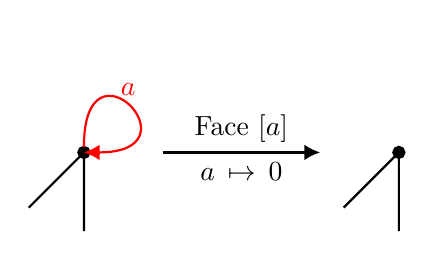
\begin{tikzpicture}[thick]
        \filldraw (0,0) coordinate(b) circle (2pt);
        \draw (-0.7,-0.7) -- (b) -- (0,-1);

        \def\off{4}
        \filldraw (\off,0) coordinate (a) circle (2pt);
        \draw ({\off-0.7},-0.7) -- (a) -- (\off,-1);

        \path  [-{Latex[length=2mm,width=2mm]},red] (b) edge [yshift=2pt,loop above,min distance=15mm,in=0,out=90,looseness=10] node [above] {$a$} (b);

        \draw [-{Latex[length=2mm,width=2mm]},thick] (1,0) --node [above] {Face $[a]$} node [below,text width=2cm,align=center] {$a\mapsto 0$} ({\off-1},0);
    \end{tikzpicture}
    }
    \hspace{1cm}
    \scalebox{\scale}{
    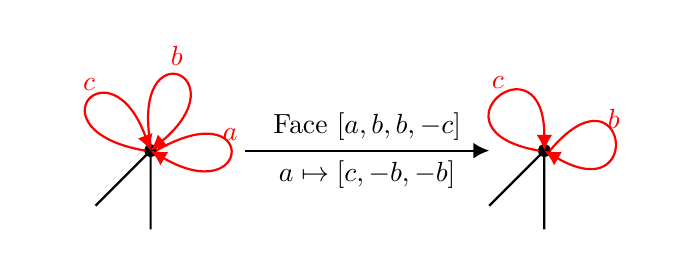
\begin{tikzpicture}[thick]
        \filldraw (0,0) coordinate(b) circle (2pt);
        \draw (-0.7,-0.7) -- (b) -- (0,-1);

        \path  [-{Latex[length=2mm,width=2mm]},red] (b) edge [xshift=2pt,loop above,min distance=15mm,in=-30,out=30,looseness=10] node [above] {$a$} (b);
        \path  [-{Latex[length=2mm,width=2mm]},red] (b) edge [yshift=2pt,loop above,min distance=15mm,in=40,out=100,looseness=10] node [above] {$b$} (b);
        \path  [-{Latex[length=2mm,width=2mm]},red] (b) edge [xshift=-2pt,loop above,min distance=15mm,in=110,out=170,looseness=10] node [above] {$c$} (b);

        \def\off{5}
        \filldraw (\off,0) coordinate (a) circle (2pt);
        \draw ({\off-0.7},-0.7) -- (a) -- (\off,-1);

        \path  [-{Latex[length=2mm,width=2mm]},red] (a) edge [xshift=2pt,loop above,min distance=15mm,in=-30,out=50,looseness=10] node [above] {$b$} (a);
        \path  [-{Latex[length=2mm,width=2mm]},red] (a) edge [xshift=-2pt,loop above,min distance=15mm,in=90,out=170,looseness=10] node [above] {$c$} (a);

        \draw [-{Latex[length=2mm,width=2mm]},thick] (1.2,0) -- node [above] {Face $[a,b,b,-c]$} node [below] {$a\mapsto [c,-b,-b]$} ({\off-0.7},0);
    \end{tikzpicture}
    }
    \par\bigskip

    \scalebox{\scale}{
    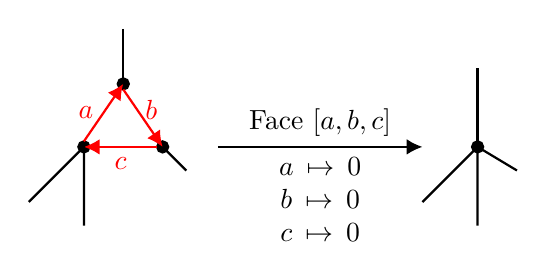
\begin{tikzpicture}[thick]
        \filldraw (0,0) coordinate (a) circle (2pt);
        \filldraw (0.5,0.8) coordinate (b) circle (2pt);
        \filldraw (1,0) coordinate (c) circle (2pt);

        \path  [-{Latex[length=2mm,width=2mm]},red] (a) edge [yshift=2pt] node [above,left] {$a$} (b);
        \path  [-{Latex[length=2mm,width=2mm]},red] (b) edge [yshift=-2pt] node [yshift=3pt,xshift=3pt] {$b$} (c);
        \path  [-{Latex[length=2mm,width=2mm]},red] (c) edge [xshift=-2pt]  node [below] {$c$} (a);


        \draw (-0.7,-0.7) -- (a) -- (0,-1);
        \draw (1.3,-0.3) -- (c);
        \draw (0.5,1.5) -- (b);

        \def\off{5}

        \begin{scope}[shift={(\off,0)}]
            \filldraw (0,0) circle (2pt);
            \draw (-0.7,-0.7) -- (0,0) -- (0,-1);
            \draw (0.5,-0.3) -- (0,0);
            \draw (0,1) -- (0,0);
        \end{scope}


        \draw [-{Latex[length=2mm,width=2mm]},thick] (1.7,0) -- node [above] {Face $[a,b,c]$} node [below,text width=2cm,align=center] {$a\mapsto 0$\\$b\mapsto 0$\\$c\mapsto 0$} ({\off-0.7},0);
    \end{tikzpicture}
    }
    \hspace{1cm}
    \scalebox{\scale}{
    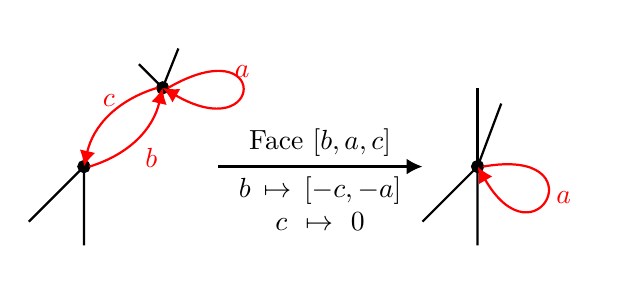
\begin{tikzpicture}[thick]
        \filldraw (0,0) coordinate(a) circle (2pt);
        \filldraw (1,1) coordinate(b) circle (2pt);
        \draw (-0.7,-0.7) -- (a) -- (0,-1);
        \draw (0.7,1.3) -- (b) -- (1.2,1.5);

        \path  [-{Latex[length=2mm,width=2mm]},red] (b) edge [xshift=2pt,loop above,min distance=15mm,in=-30,out=30,looseness=10] node [above] {$a$} (b);
        \path  [-{Latex[length=2mm,width=2mm]},red] (a) edge [bend right,xshift=2pt]  node [below,xshift=5pt] {$b$} (b);
        \path  [-{Latex[length=2mm,width=2mm]},red] (b) edge [bend right,xshift=-2pt] node [above] {$c$} (a);

        \def\off{5}

        \begin{scope}[shift={(\off,0)}]
            \filldraw (0,0) coordinate (c) circle (2pt);
            \draw (-0.7,-0.7) -- (c) -- (0,-1);
            \draw (0.3,0.8) -- (c);
            \draw (0,1) -- (c);

            \path  [-{Latex[length=2mm,width=2mm]},red] (c) edge [xshift=2pt,loop above,min distance=15mm,in=-60,out=10,looseness=10] node [right] {$a$} (c);
        \end{scope}


        \draw [-{Latex[length=2mm,width=2mm]},thick] (1.7,0) -- node [above] {Face $[b,a,c]$} node [below,text width=3cm,align=center] {$b\mapsto [-c,-a]$\\$c\mapsto 0$} ({\off-0.7},0);
    \end{tikzpicture}
    }
    \caption{From top left to bottom right, examples for Case $2.1$, $3$, $2.2$ and $4$. The Face is described above the arrow, the resulting additional mappings of edges is described below the arrow.}
	\label{contractions}
\end{figure}

    \section{Distance Measures}\label{ch:distance-measures}

    First of all we want to extend the Wasserstein distance to differently sized sets.
    A first idea was to minimize $\varphi:X\rightarrow Y$ for $|X|<|Y|$ via injections $\varphi:X\rightarrow Y$, and to introduce an error term for every point in $Y$ that is not hit.
    This seemed promising.\\
    Define $\gamma:\bR^2\rightarrow\bR$, with $(x,y)\mapsto y-x$.
    The motivation behind this definition is that this is exactly the vertical distance from a point $(x,y)$ to the diagonal.
    Then we define \[W_p'(X,Y):=\min_{\varphi:X\rightarrow Y}\left(\sum_{x\in X}|||x-\varphi(x)||^p + \sum_{y\in Y\setminus \in(\varphi)}\gamma(y)^p\right)^\frac{1}{p}.\]
    This approach seemed promising at first, but the error term was too big.
    The problem is that $||x-\varphi(x)||$ is the $\ell_2$ norm from the distance of $x$ and $\varphi(x)$, whereas $\gamma(y)$ is the $\ell_1$ norm from the distance of $y$ and $\Delta$.
    If you define $\gamma(x,y)=\frac{y-x}{\sqrt{2}}$ instead, you get a fair distribution.
    However we noticed that this distance is too restrictive.
    We also want to allow points from $X$ not to be mapped.
    So now we define the final version of our modified Wasserstein distance, where we apply the error term to any point from $X$ that is not mapped, as well as any point from $Y$ that is not hit.
    \[V_p(X,Y):=\min_{Z\subset{X}}\min_{\varphi:Z\rightarrow Y}\left(\sum_{z\in Z}||z-\varphi(z)||^p + \sum_{y\in (Y\setminus \im(\varphi))\cup X\setminus Z}\gamma(y)^p\right)^\frac{1}{p}.\]

    We call the bottleneck distance $B(X,Y) := V_\infty(X,Y)$.
    Since we now have three different Wasserstein distances, we want to make clear, the $V_p(\_,\_)$ will be the distance in question from now on.\\
    In Figure \ref{distances} is an example of all the different distances, a single point from the set $X$ has to consider. We want to find a mapping the reduces the sum of the selected lengths, or the maximum such length respectively.
     \begin{figure}
    	\centering
    	\fbox{
    		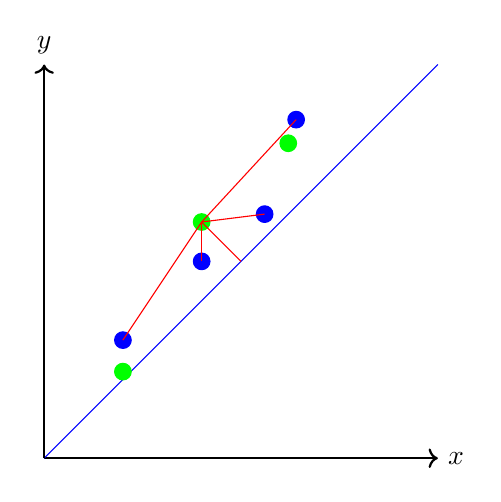
\begin{tikzpicture}
    		% Achsen zeichnen
    		\draw[->,thick] (0,0) -- (5,0) node[right] {$x$};
    		\draw[color=blue] (0,0) -- (5,5);
    		\draw[->,thick] (0,0) -- (0,5) node[above] {$y$};
    		%Punkte einzeichnen:
    		\filldraw[color=green] (2,3) coordinate(a) circle (3pt);
    		\filldraw[color=green] (1,1.1) coordinate(b) circle (3pt);
    		\filldraw[color=green] (3.1,4) coordinate(c) circle (3pt);
    		
    		\filldraw[color=blue] (1,1.5) coordinate(d) circle (3pt);
    		\filldraw[color=blue] (2,2.5) coordinate(e) circle (3pt);
    		\filldraw[color=blue] (2.8,3.1) coordinate(f) circle (3pt);
    		\filldraw[color=blue] (3.2,4.3) coordinate(g) circle (3pt);
    		
    		\draw[red] (2.5,2.5) -- (a);
    		
    		\draw[red] (d) -- (a);
    		\draw[red] (e) -- (a);
    		\draw[red] (f) -- (a);
    		\draw[red] (g) -- (a);
    		
    		\end{tikzpicture}
    	}
    	\caption{\textit{The second homology of two different persistence Diagrams in green and blue. Red are all the different distances, a single point of the green diagram has to consider in the mapping problem.}}
    	\label{distances}
    \end{figure}

    \subsection{Efficient Calculation}\label{sec:efficient-calculation}

    We quickly noticed that the whole problem is closely related to the Optimal Mapping problem.
    We want to make use of the knowledge we have of the ''Optimal Mapping'' problem and present the problem of minimizing over exponentially many mappings as a flow problem.
    So for $V_p(X,Y)$ we define the following graph. $V := X\cup Y\cup {s,t,h,h'}$ and $E := (X\cup h)\times (Y\cup h') \cup {s}\times (X\cup h) \cup (Y\cup h')\times t$.\\
    \begin{figure}
        \centering
        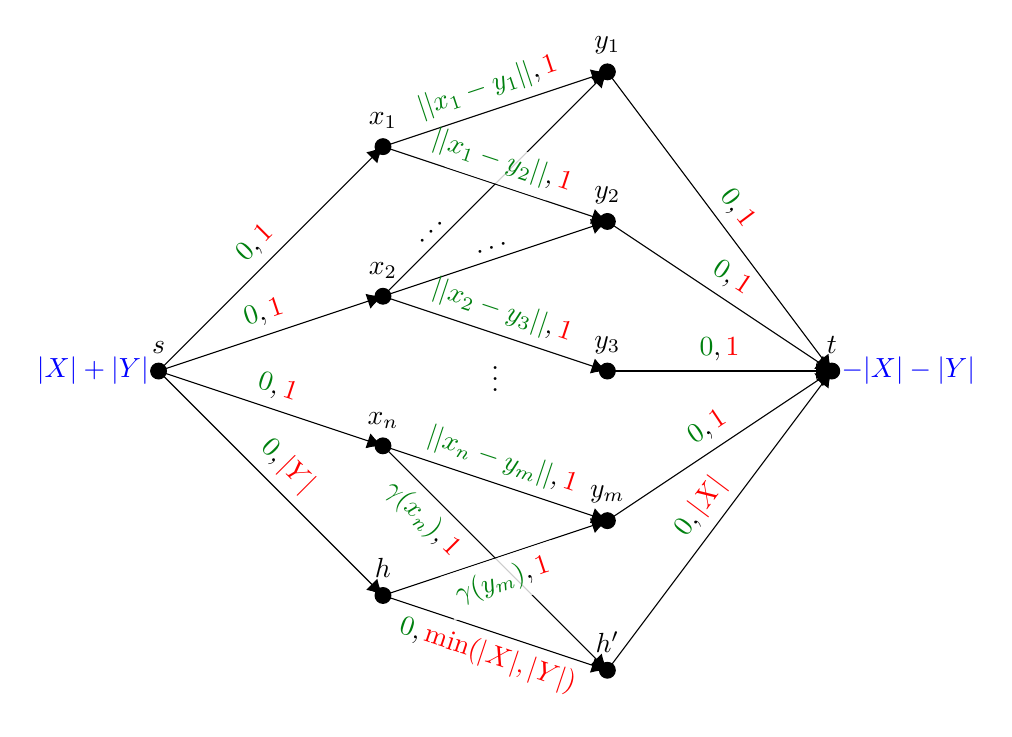
\begin{tikzpicture}[scale = .95]
            \definecolor{mycolor}{rgb}{0, 0.500, 0.06};
            \definecolor{red}{rgb}{1,0,0};
            \definecolor{blue}{rgb}{0,0,1};
            \filldraw (0,0) coordinate(s) circle (3pt);
            \node at (s) [above = 1mm of s] {$s$};
            \node at (s) [left,blue] {$|X|+|Y|$};

            \filldraw (3,3) coordinate(x1) circle (3pt);
            \node at (x1) [above = 1mm of x1] {$x_1$};
            \filldraw (3,1) coordinate(x2) circle (3pt);
            \node at (x2) [above = 1mm of x2] {$x_2$};
            \filldraw (3,-1) coordinate(x3) circle (3pt);
            \node at (x3) [above = 1mm of x3] {$x_n$};
            \filldraw (3,-3) coordinate(h) circle (3pt);
            \node at (h) [above = 1mm of h] {$h$};



            \filldraw (6,4) coordinate(y1) circle (3pt);
            \node at (y1) [above = 1mm of y1] {$y_1$};
            \filldraw (6,2) coordinate(y2) circle (3pt);
            \node at (y2) [above = 1mm of y2] {$y_2$};
            \filldraw (6,0) coordinate(y3) circle (3pt);
            \node at (y3) [above = 1mm of y3] {$y_3$};
            \filldraw (6,-2) coordinate(y4) circle (3pt);
            \node at (y4) [above = 1mm of y4] {$y_m$};
            \filldraw (6,-4) coordinate(hs) circle (3pt);
            \node at (hs) [above = 1mm of hs] {$h'$};

            \filldraw (9,0) coordinate(t) circle (3pt);
            \node at (t) [above = 1mm of t] {$t$};
            \node at (t) [right,blue] {$-|X|-|Y|$};

            \draw [-{Latex[length=2mm,width=2mm]}] (s) -- (x1) node [midway,above, sloped] {$\textcolor{mycolor}{0},\textcolor{red}{1}$};
            \draw [-{Latex[length=2mm,width=2mm]}] (s) -- (x2) node [midway,above, sloped] {$\textcolor{mycolor}{0},\textcolor{red}{1}$};
            \draw [-{Latex[length=2mm,width=2mm]}] (s) -- (x3) node [midway,above, sloped] {$\textcolor{mycolor}{0},\textcolor{red}{1}$};
            \draw [-{Latex[length=2mm,width=2mm]}] (s) -- (h) node [midway,above, sloped] {$\textcolor{mycolor}{0},\textcolor{red}{|Y|}$};


            \draw [-{Latex[length=2mm,width=2mm]}] (x1) -- (y1) node [midway,above, sloped] {$\textcolor{mycolor}{||x_1-y_1||},\textcolor{red}{1}$};
            \draw [-{Latex[length=2mm,width=2mm]}] (x2) -- (y1) node [midway,near start,sloped,above] {$\ldots$};
            \draw [-{Latex[length=2mm,width=2mm]}] (x1) -- (y2) node [midway,above, sloped,fill=white,fill opacity = 0.8,color=white] {$x_1-y_2$}node [midway,above, sloped] {$\textcolor{mycolor}{||x_1-y_2||},\textcolor{red}{1}$};
            \draw [-{Latex[length=2mm,width=2mm]}] (x2) -- (y2)node [midway,sloped,above] {$\ldots$};
            \draw [-{Latex[length=2mm,width=2mm]}] (x2) -- (y3)node [midway,above, sloped] {$\textcolor{mycolor}{||x_2-y_3||},\textcolor{red}{1}$};

            \node at (4.5,0) {$\vdots$};

            \draw [-{Latex[length=2mm,width=2mm]}] (x3) -- (y4) node [midway,above, sloped] {$\textcolor{mycolor}{||x_n-y_m||},\textcolor{red}{1}$};
            \draw [-{Latex[length=2mm,width=2mm]}] (x3) -- (hs) node [midway,near start,below, sloped] {$\textcolor{mycolor}{\gamma(x_n)},\textcolor{red}{1}$};
            \draw [-{Latex[length=2mm,width=2mm]}] (h) -- (hs) node [midway,below, sloped] {$\textcolor{mycolor}{0},\textcolor{red}{\min(|X|,|Y|)}$};
            \draw [-{Latex[length=2mm,width=2mm]}] (h) -- (y4)node [midway,below, sloped,fill=white,fill opacity = 0.8, color=white] {$\gamma(y_m),1$}  node [midway,below, sloped] {$\textcolor{mycolor}{\gamma(y_m)},\textcolor{red}{1}$};



            \draw [-{Latex[length=2mm,width=2mm]}] (y1) -- (t) node [midway,above, sloped] {$\textcolor{mycolor}{0},\textcolor{red}{1}$};
            \draw [-{Latex[length=2mm,width=2mm]}] (y2) -- (t) node [midway,above, sloped] {$\textcolor{mycolor}{0},\textcolor{red}{1}$};
            \draw [-{Latex[length=2mm,width=2mm]}] (y3) -- (t) node [midway,above, sloped] {$\textcolor{mycolor}{0},\textcolor{red}{1}$};
            \draw [-{Latex[length=2mm,width=2mm]}] (y4) -- (t) node [midway,above, sloped] {$\textcolor{mycolor}{0},\textcolor{red}{1}$};
            \draw [-{Latex[length=2mm,width=2mm]}] (hs) -- (t) node [midway,above, sloped] {$\textcolor{mycolor}{0},\textcolor{red}{|X|}$};

            %\draw [-{Latex[length=2mm,width=2mm]},color=red] (a) -- (b) node[midway,below,sloped,color=black]{a};
            %\draw [-{Latex[length=2mm,width=2mm]},color=red](a) -- (c)node[midway,below,sloped,color=black]{b};
            %\draw [-{Latex[length=2mm,width=2mm]},color=red](b) -- (c)node[midway,above,sloped,color=black]{c};

            %\draw[-{Latex[length=2mm,width=2mm]}] (a) -- (d)node[midway,below,sloped,color=black]{d};
            %\draw[-{Latex[length=2mm,width=2mm]}] (d) -- (e)node[midway,below,sloped,color=black]{e};
            %\draw[-{Latex[length=2mm,width=2mm]}] (e) -- (f)node[midway,below,sloped,color=black]{f};
            %\draw[-{Latex[length=2mm,width=2mm]}] (f) -- (g)node[midway,below,sloped,color=black]{g};
            %\draw[-{Latex[length=2mm,width=2mm]}] (g) -- (h)node[midway,below,sloped,color=black]{h};
            %\draw[-{Latex[length=2mm,width=2mm]}] (b) -- (h)node[midway,below,sloped,color=black]{i};
        \end{tikzpicture}
        \caption{Structure of the constructed graph.
        Flow requirements are blue, capacities red and costs green.}
        \label{graph}
    \end{figure}

    Weights are selected as follows.
    For edges in ${s}\times (X\cup h) \cup (Y\cup h')\times t \cup \{(h,h')\}$ they are always 0.
    For edges of the form $(x,y)\in X\times Y$ the costs are exactly $||x-y||$, and for edges of the form $(x,h')\in X\times \{h'\}$ resp. $(h,y)\in \{h\}\times Y$ we select $\gamma(x)$ or $\gamma(y)$.
    As capacities we choose $|Y|,|Y|$ and $\min(|X|,|Y|)$ for $(s,h),(h',t)$ and $(h,h')$ respectively and $1$ for all other edges.
    And finally the flow requirements $b(s) = -b(t) = |X|+|Y|$, and $b(v)=0$ for all others. 
    In Figure \ref{graph} one can see the structure of the constructed graph.\\ 
    In order to solve the Wasserstein distance via a min-cost flow instance, we must first prove that for every feasible integer flow there is a $Z\subset X$ and map $\varphi:Z\rightarrow Y$, where the cost of the flow is equal to the error term of $\varphi$ and vice versa.
    From this it follows that the cost of a min-cost-flow is equal to the Wasserstein distance.
    Note that this cost only applies to $p=1$.
    For $1<p<\infty$ exponentiate the cost of all edges by $p$ and return the $p$th root of the cost at the end.

    \begin{lemma}
        The cost of a min-cost-flow for the above graph $G=(V,E)$ is equal to the Wasserstein distance $V_p(X,Y)$.
    \end{lemma}
    \begin{proof}
        Let $f:E\rightarrow \bZ_{\geq0}$ be a feasible flow.
        For $Z$ choose all vertices $x$ from $X$, such that $f((x,y))=1$ for a $y\in Y$ and set $\varphi(x) = y$ for this y.
        In less mathy terms, $\varphi$ is given by the selected flow edges of $f$, between $X$ and $Y$.
        Since the cost of the edges of the form $(x,h')$ or $(h,y)$ selected by the flow is exactly $\gamma(x)$ and $\gamma(y)$, $V_p(X,Y)$ is a lower bound for the min-cost-flow value.\\
        For the other direction we consider for given $Z,\varphi$ the flow given by $f(x,y)=1$ iff $x\in Z$ and$ \varphi(x)=y$.
        For all $x\in X\setminus Z$ we set $f((x,h'))=1$ and for $y\in Y\setminus \im(\varphi)$ we set $f((h,y))=1$.
        Thus one receives a feasible flow, with the same costs.
    \end{proof}

    And as we know, the min-cost-flow problem can be calculated in polynomial time with an algorithm like Edmonds-Karp.\\
    To calculate the Bottleneck distance, we consider the subgraph given by all edges with weights smaller than a given value.
    Since the Bottleneck distance is given by the cheapest edge, so that with all cheaper edges a feasible flow is still possible, one can determine the Bottleneck distance with logarithmically many calls of a min-cut algorithm with a procedure like binary search.
    This reduction follows from the fact, that the error term that is to be minimized in the Wasserstein distance is the same as the $p$-norm.
    The Bottleneck distance hence is the same as the $\infty$-norm, and is described by the maximum.
    Hence the Bottleneck distance reduces to finding the value $$\min_{\varphi:Z\subset X \rightarrow Y} \max\bigg(\max_{x\in Z}||x - \varphi(x)||,\max_{y\in Y\setminus\im\varphi\cup X\setminus Z}\gamma(y)\bigg).$$\\
    This leaves us with the following approximations for runtime.
    Let $X$ and $Y$ again be arbitrary.
    Then the graph consists of $n=2+|X|+|Y|$ vertices and $m=3+2|X|+2|Y|+|X||Y|$ edges.
    Assuming a runtime of $O(n^2m)$ for Dinic's algorithm, we have a runtime of $O(|X||Y|^3 + |X|^3|Y|)$ for the Wasserstein distance.
    For the Bottleneck distance we get a runtime of $O((\log(|X||Y|))(|X||Y|^3 + |X|^3|Y|))$.
    Note that Dinic's Algorithm is not necessarily the fastest for this type of problem, since the very easy structure of the graph opens the door to more specialized algorithms.

    \section{Feature Proposals}\label{ch:feature-proposals}
    To combine all of this to actually calculate a distance of two images, we need to reduce an image to a pointset. For this we looked at different typed of feature detection algorithms and compared these.
    \subsection{Feature Detection}\label{sec:feature-detection}
    To do this we first considered an image, converted it to grayscale and then tried out existing feature detection algorithms.
    We tested the Laplace operator, the Harris operator and Canny edge detection.\\
    The Laplace operator computes the 2nd spatial derivative and therefore may output many different gray values for one image, which is less usable for our approach.
    That is because we are trying to represent image structures with points, which is not possible to do in an accurate manner, if the feature detection outputs only a ''probability'' for an edge or corner.\\
    Next up is the harris operator, which highlights corners inside an image.
    One could think, that this is exactly what we need, but in fact we need to describe lines as series of points and not only start and end point.
    That rules out the Harris operator for our case as well.\\
    Finally we tested the Canny operator, which only outputs either 0 or 1 for each pixel, given a threshold.
    Its used for edge detection and given the previous explanation exactly what we need.
    There might be some dynamic threshold computation left to do, so that the user doesn't have to choose that parameter on its own.
    \subsection{Feature Selection}\label{sec:feature-selection}
    Now we have a feature detection, that outputs a bitmap with ones for all edges in the image.
    The next thing to do is to convert that bitmap into 2D points, that will be used to compute the persistent homology.
    The idea beneath the used algorithm is inspired by Poisson-Disc sampling and works as follows:
    We sample the area above threshold by adding random white points, that are at least twice a given radius away from all other samples.
    That way we have control over the granularity of the sampling using only a radius parameter.
    The given space between each sample also ensures, that the numerical accuracy of the Voronoi algorithm does not have to be that exact.
    \lstset{language=Java}
\begin{figure}
    \begin{lstlisting}[frame=single]
        public static List<PointD> sample(Mat matrix, int radius) {
            List<PointD> points = new ArrayList<>();
            // Create a "white" 2D point for each pixel above a given threshold
            ...
            List<PointD> samples = new ArrayList<>();
            while (!points.isEmpty()) {
                // Add a random white point to the samples and remove all white points within twice a given radius of the new sample
                int index = (int) (Math.random() * points.size());
                PointD sample = points.remove(index);
                samples.add(sample);
                points.removeIf(point -> point.subtract(sample).length() < 2 * radius);
            }
            ...
            return samples;
        }
    \end{lstlisting}
    \caption{\textit{Codesnippet of the sampling algorithm}}
    \label{fig8}
\end{figure}
    \section*{Conclusion}\addcontentsline{toc}{section}{Conclusion}
    In this work we have presented two different ways to compute the persistent Homology of a given $2$-dimensional point set. We began with a very na\"ive way, where we simply built up a big matrix, and continuously solved it for its kernel, and then used information from the kernel to reduce the size of the matrix. The second approach was much more involved, and made changes to the underlying graph, to keep the complexity of the problem small from the very beginning.\\
    We then used the calculated persistent Homology, to compute their difference. For this we changed the Wasserstein- and Bottleneck-distances to also accept differently sized point sets, and made this changes in a way, that it respects the significance of the underlying data - namely the persistent homology.\\
    To compute this, we reduced the problem to a flow-instance, and showed, that the distances can be computed in polynomial time. Namely for $|X|=n$ and $|Y|=m$ we achieved a run time of $O(nm^3+n^3m)$ and $O(\log(nm)(nm^3+n^3m))$ respectively.\\
    To put all of this to use, we presented some already well-known methods, to reduce an input image to a set of points, that represent the shape of the object in the image well. We also presented a method, of how to reduce the size of these point sets to increase the speed of our method without loosing much of the accuracy.\\
    An important limitation however is, that this handcrafted approach really only works well with $2$-dimensional data. It would be interesting to see, if there is a similar approach to the contractions on the graph for higher dimensional input data/a Čech-Complex with higher non-trivial homologies.
    %TODO Whoever
    %TODO Symbol table? Proper chapter elevation? Conclusion own page? Kapitel -> Chapter? ...
    %TODO Konsistenz (Rechtschreibung)
   

\end{document}